\chapter{मिलाना और घुलना}\label{ch:g2:mixing-and-dissolving}

गरम चाय के प्याले में चीनी का एक घन गिरता है। चम्मच चलता है, घन
भुरभुरा होकर बिखर जाता है, और थोड़ी देर बाद कुछ भी दिखाई नहीं देता:
चाय बिल्कुल पहले जैसी दिखती है। फिर भी अब चाय मीठी लगती है। चीनी कहीं
गई नहीं --- वह चाय में छिपी है। यह अध्याय चीज़ों को एक साथ मिलाने के
बारे में है, और उन चीज़ों के बारे में जो मिलाने पर ग़ायब-सी हो जाती हैं।

\begin{omfigure}
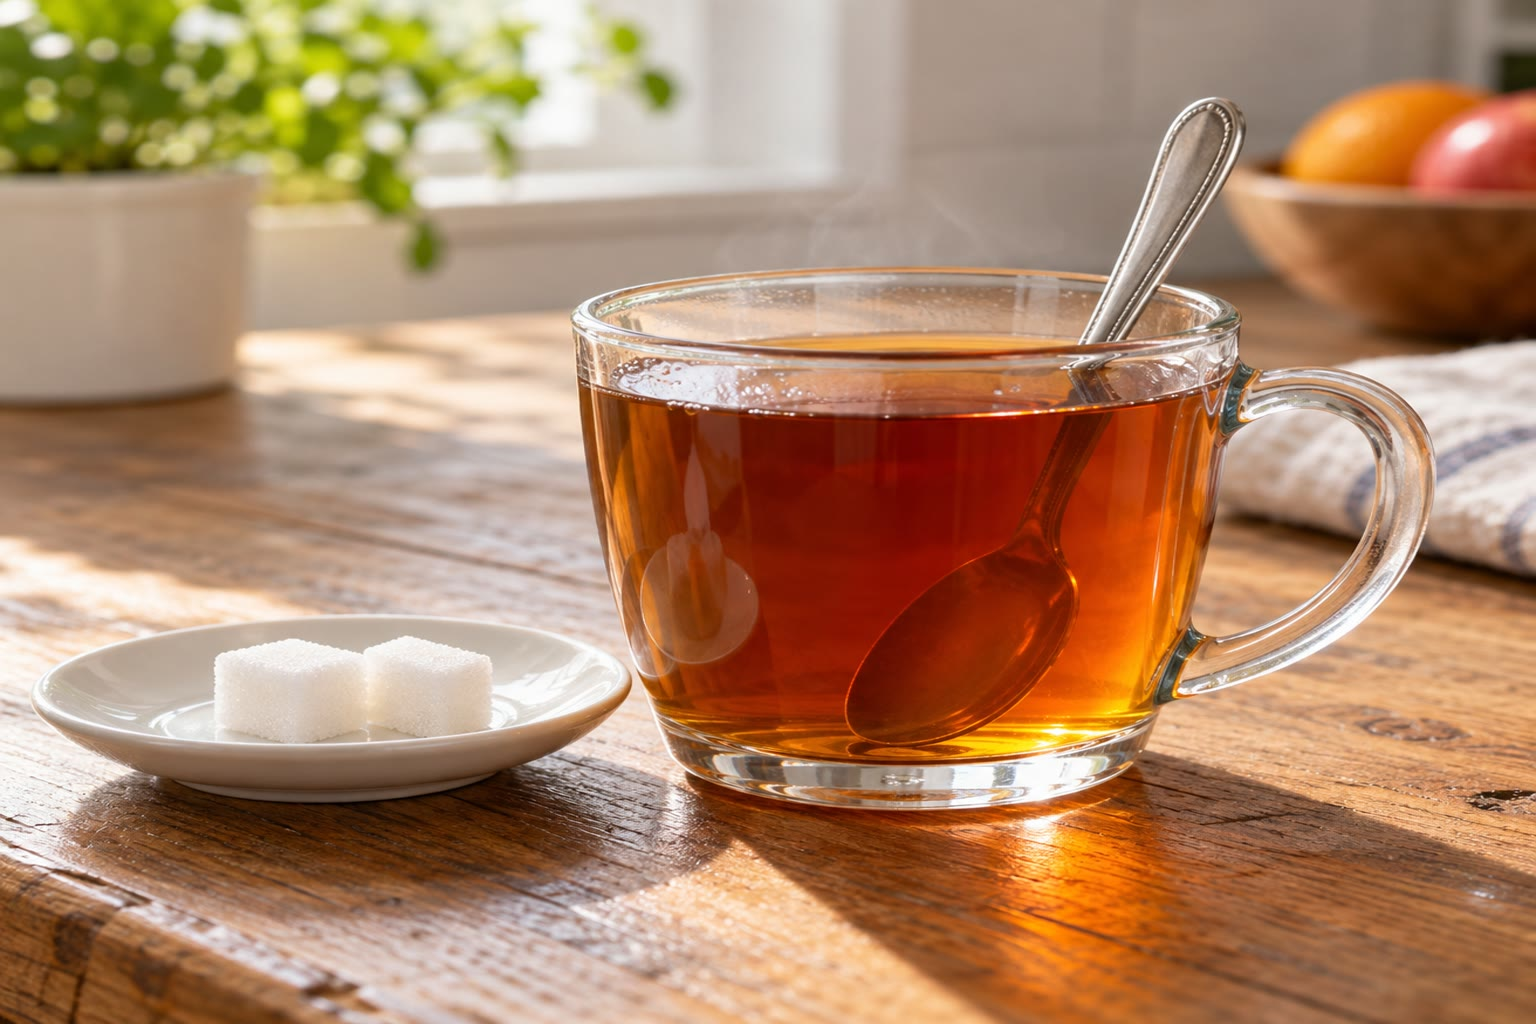
\includegraphics[width=0.55\linewidth]{images/book1/ai/g2-tea-sugar.jpg}

{\small चाय का एक प्याला और चीनी के दो घन। घोलने पर चीनी आँखों से
ओझल हो जाती है, पर स्वाद से नहीं।}
\end{omfigure}

\section{चीज़ों को एक साथ मिलाना}

\begin{definition}[मिलाना]\label{def:g2:mixing-and-dissolving:mix}
\emph{मिलाना}\index{मिलाना} यानी अलग-अलग चीज़ों को एक साथ रखना, और
अक्सर उन्हें चलाना भी। जो हमें मिलता है, वह उन चीज़ों का मिश्रण होता है।
\end{definition}

\begin{example}[मूसली की कटोरी]\label{ex:g2:mixing-and-dissolving:muesli}
जई, किशमिश, मेवे और बीज एक ही कटोरी में डाले जाते हैं: यह एक मिश्रण है।
ध्यान से देखो तो हर चीज़ अब भी दिखती है और उँगलियों से फिर से बीनी
जा सकती है --- किशमिश किशमिश ही रहती है, मेवा मेवा ही रहता है।
\end{example}

\begin{example}[पानी में शरबत]\label{ex:g2:mixing-and-dissolving:syrup}
दो द्रव भी मिलाए जा सकते हैं। पानी के गिलास में डाला गया लाल शरबत रंग
के छल्ले बनाता हुआ नीचे बैठता है; चम्मच चलाने पर पूरा गिलास एक-सा
गुलाबी हो जाता है। अब आँख से शरबत और पानी को अलग-अलग नहीं पहचाना जा सकता।
\end{example}

\begin{omfigure}
\begin{minipage}[t]{0.48\linewidth}\centering
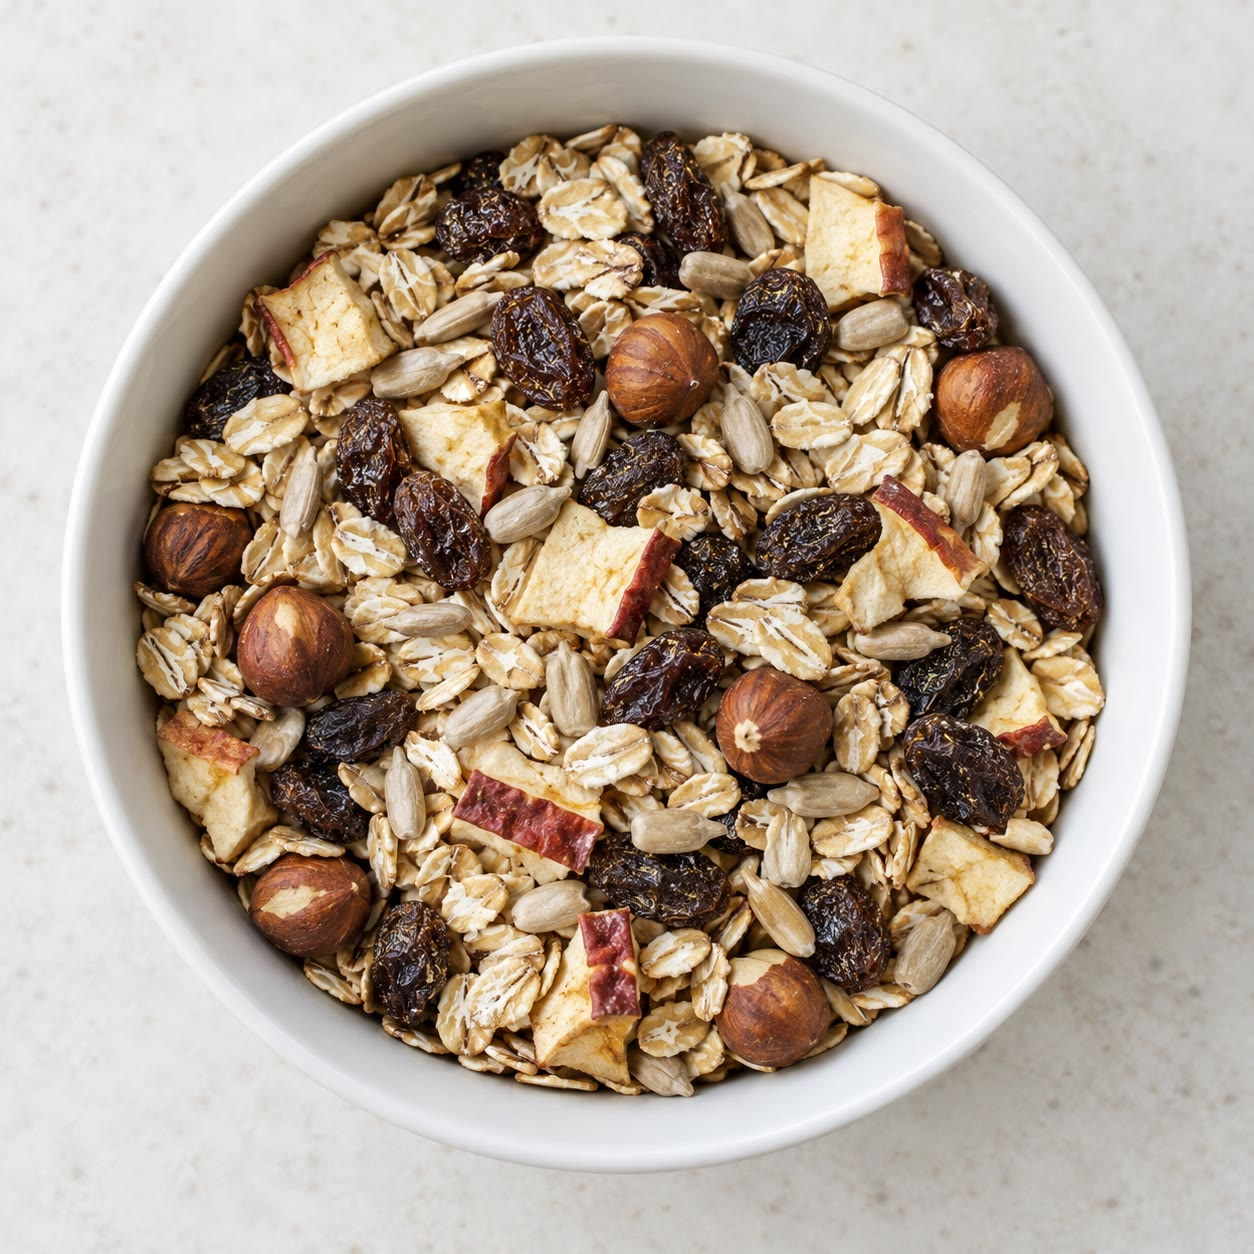
\includegraphics[width=\linewidth,height=4.6cm,keepaspectratio]{images/book1/ai/g2-muesli.jpg}

{\small मूसली: ऐसा मिश्रण जिसका हर हिस्सा अब भी दिखता है।}
\end{minipage}\hfill
\begin{minipage}[t]{0.48\linewidth}\centering
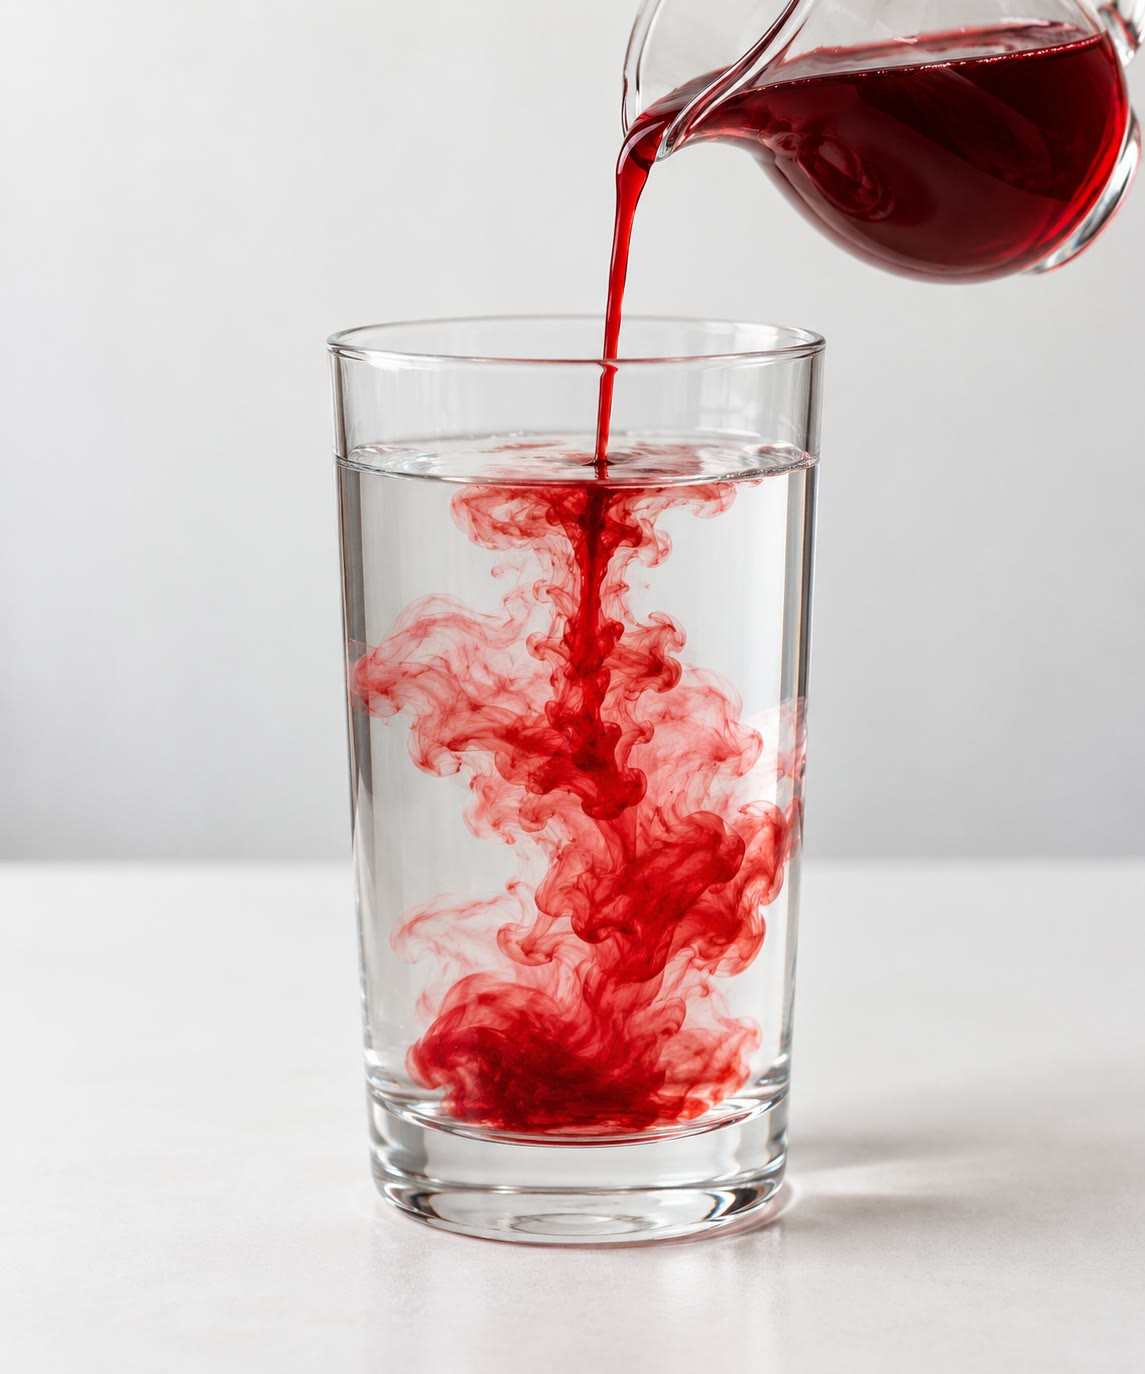
\includegraphics[width=\linewidth,height=4.6cm,keepaspectratio]{images/book1/ai/g2-syrup-in-water.jpg}

{\small पानी में डाला गया शरबत: दो द्रव आपस में मिल रहे हैं।}
\end{minipage}
\end{omfigure}

\begin{remark}[मिलाने से कुछ नष्ट नहीं होता]\label{rem:g2:mixing-and-dissolving:nothing-lost}
चीज़ों को मिलाने पर न कुछ खोता है, न कुछ नया बनता है। जई, किशमिश और
मेवे सब अब भी कटोरी में हैं। आगे का एक अध्याय दिखाता है कि मिश्रण को
फिर से अलग-अलग कैसे किया जाता है।
\end{remark}

\section{घुलने वाली चीज़ें}

\begin{definition}[घुलना और विलयन]\label{def:g2:mixing-and-dissolving:dissolve}
कोई ठोस पानी में \emph{घुलता}\index{घुलना} है, जब पानी में मिलाकर
चलाने पर वह आँखों से ओझल हो जाता है और द्रव को \emph{स्वच्छ}, यानी
आर-पार दिखने वाला, छोड़ देता है। चीनी और नमक पानी में घुलते हैं।
इस तरह मिलने वाले स्वच्छ द्रव को
\emph{विलयन}\index{विलयन} कहते हैं: चीनी का पानी चीनी का विलयन है,
नमकीन पानी नमक का विलयन।
\end{definition}

\begin{example}[पानी के गिलास में चीनी का घन]\label{ex:g2:mixing-and-dissolving:cube}
शांत पानी से भरे गिलास की तली में चीनी का एक घन रखा जाता है। उसके
कोने नरम पड़ते हैं, वह छोटा होता जाता है, और उससे लहरदार धारियाँ पानी
में ऊपर उठती हैं। अगर हम चलाएँ, तो एक मिनट में वह ग़ायब हो जाता है।
अगर न चलाएँ, तब भी वह ग़ायब होता है, बस बहुत धीरे-धीरे।
\end{example}

\begin{remark}[स्वच्छ का अर्थ रंगहीन नहीं]\label{rem:g2:mixing-and-dissolving:clear}
चाय भूरी है और शरबत वाला पानी गुलाबी, पर दोनों के आर-पार देखा जा
सकता है: दोनों स्वच्छ हैं। \omterm{def:g2:mixing-and-dissolving:dissolve}{विलयन} का रंग हो सकता है। पर \omterm{def:g2:mixing-and-dissolving:dissolve}{विलयन} में कभी
तैरते कण या तली में जमी परत नहीं होती।
\end{remark}

\begin{method}[क्या यह घुलता है?]\label{met:g2:mixing-and-dissolving:test}
यह पता करने के लिए कि कोई ठोस पानी में \omterm{def:g2:mixing-and-dissolving:dissolve}{घुलता} है या नहीं:
\begin{enumerate}
  \item उस ठोस का थोड़ा-सा हिस्सा पानी के गिलास में डालो;
  \item चलाओ, फिर कुछ मिनट रुको;
  \item गिलास के आर-पार देखो:
    \begin{itemize}
      \item स्वच्छ, और तली में कुछ नहीं: ठोस घुल गया है;
      \item धुँधला, या तली में परत: ठोस नहीं घुला है।
    \end{itemize}
\end{enumerate}
\end{method}

\section{न घुलने वाली चीज़ें}

\begin{proposition}[रेत और खड़िया नहीं घुलते]\label{prop:g2:mixing-and-dissolving:not}
बहुत-से ठोस पानी में नहीं \omterm{def:g2:mixing-and-dissolving:dissolve}{घुलते}: रेत, खड़िया, मिट्टी, कंकड़, आटा।
पानी में मिलाकर चलाने पर वे उसे धुँधला कर देते हैं; छोड़ देने पर वे
नीचे बैठकर तली में जम जाते हैं, और ऊपर का पानी फिर से साफ़ होने
लगता है। हम कितनी भी देर चलाएँ, वे कभी ग़ायब नहीं होते।
\end{proposition}

\begin{example}[गंदले पानी का मर्तबान]\label{ex:g2:mixing-and-dissolving:mud}
बगीचे की मिट्टी को पानी के मर्तबान में हिलाया जाए, तो पानी भूरा और
धुँधला हो जाता है। एक घंटे बाद मिट्टी और छोटे कंकड़ तली में गहरे रंग
की परत बनाकर पड़े होते हैं, कुछ सूखी पत्तियाँ ऊपर तैरती हैं, और बीच
का पानी बस थोड़ा-सा धुँधला रहता है। मिट्टी घुली नहीं है।
\end{example}

\begin{omfigure}
\begin{minipage}[t]{0.48\linewidth}\centering
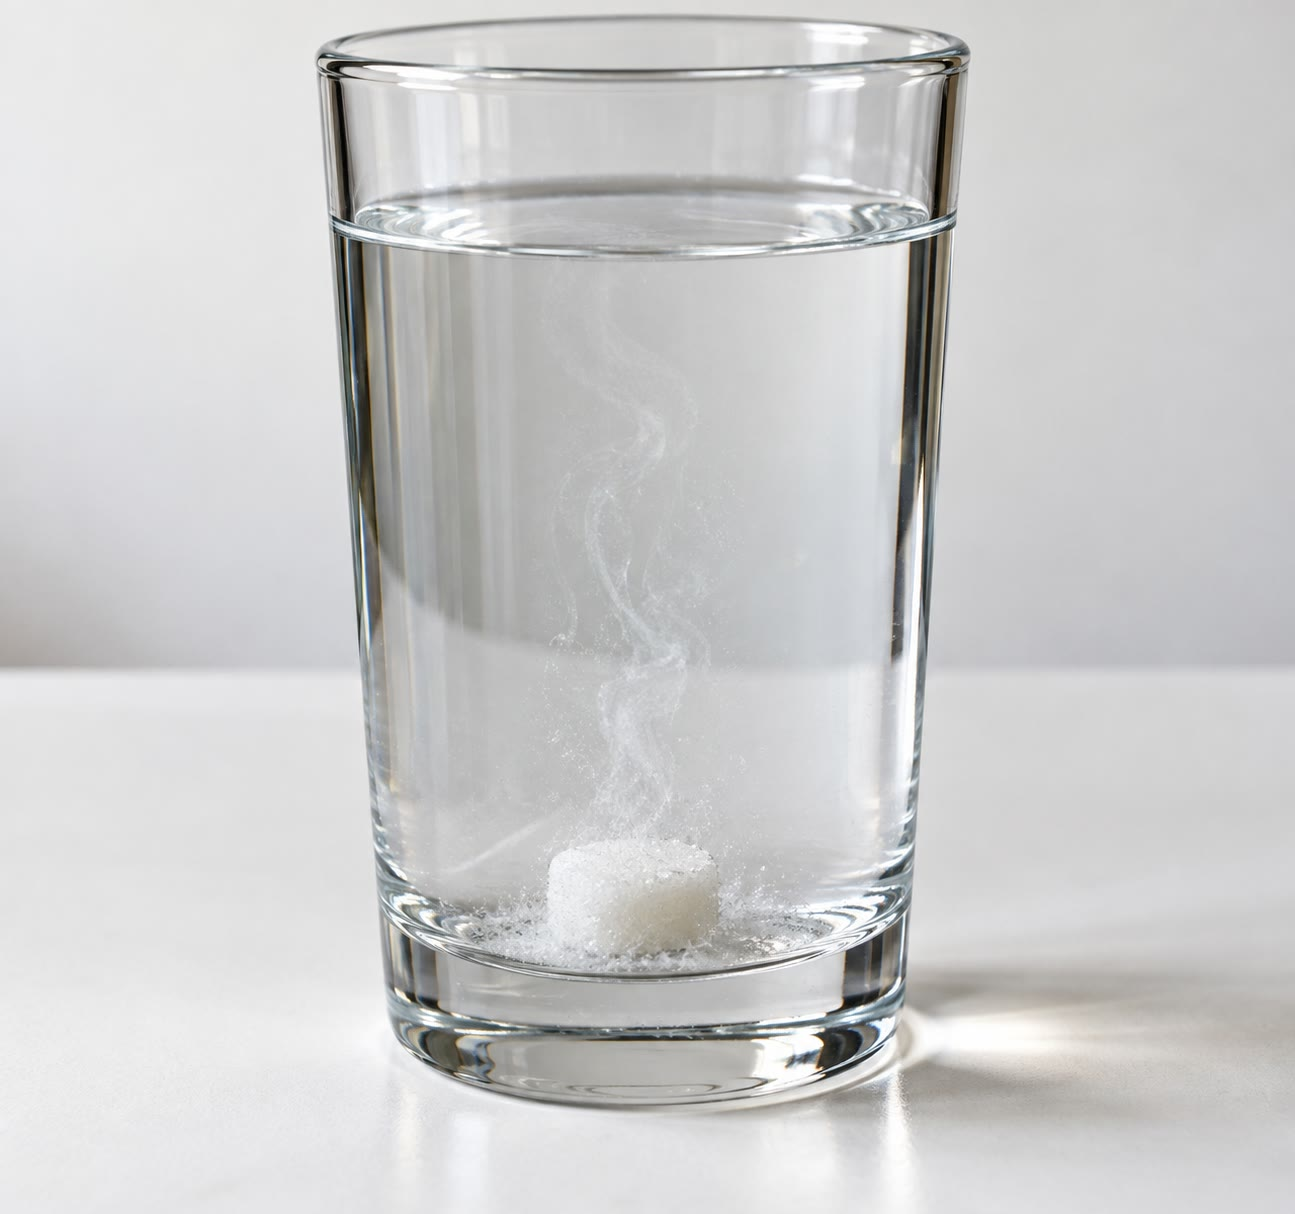
\includegraphics[width=\linewidth,height=4.6cm,keepaspectratio]{images/book1/ai/g2-sugar-cube-dissolving.jpg}

{\small चीनी घुल रही है: घन से धारियाँ ऊपर उठ रही हैं।}
\end{minipage}\hfill
\begin{minipage}[t]{0.48\linewidth}\centering
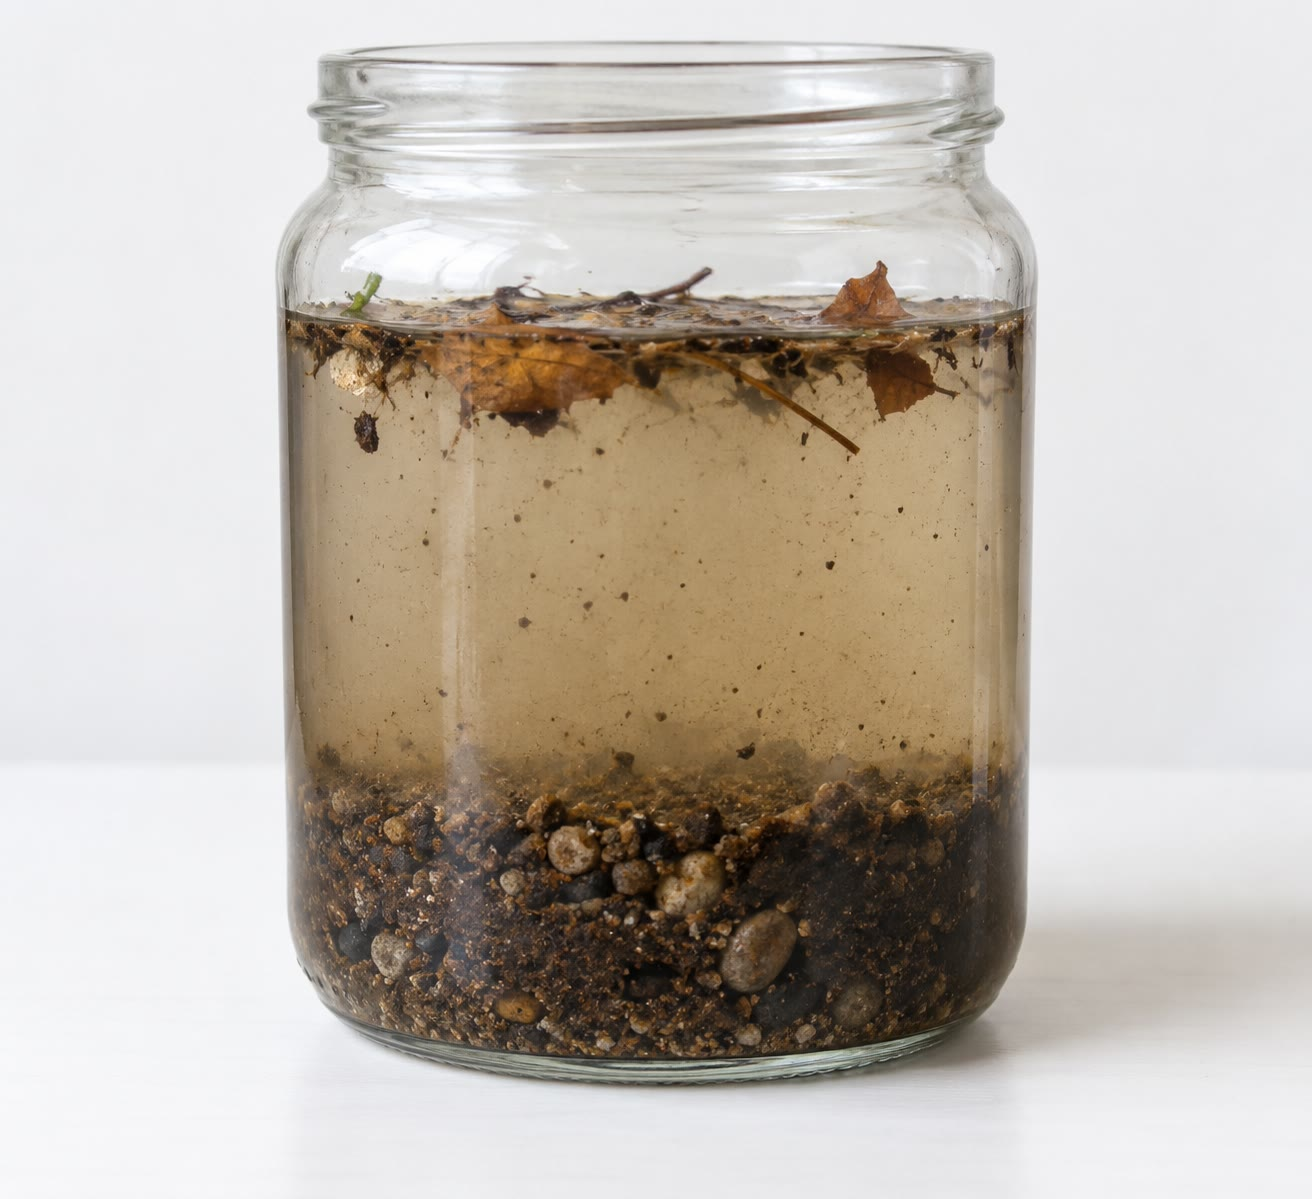
\includegraphics[width=\linewidth,height=4.6cm,keepaspectratio]{images/book1/ai/g2-muddy-jar.jpg}

{\small मिट्टी नहीं \omterm{def:g2:mixing-and-dissolving:dissolve}{घुलती}: वह तली में बैठ जाती है।}
\end{minipage}
\end{omfigure}

\begin{omfigure}
\begin{tikzpicture}[font=\small, scale=1.35]
  \pic[transform shape] at (0,0) {beaker={0.7}{omWater!70}};
  \fill[brown!55] (4.2,0) rectangle (5.8,0.22);
  \pic[transform shape] at (5,0) {beaker={0.7}{brown!12}};
  \fill[brown!55] (4.2,0) rectangle (5.8,0.22);
  \draw[omGlass, line width=0.7pt] (4.2,0.22) -- (4.2,0) -- (5.8,0) -- (5.8,0.22);
  \foreach \x/\y in {4.4/0.32,4.75/0.45,5.1/0.3,5.5/0.5,4.6/0.7,5.3/0.8,4.9/1.0}
    \fill[brown!60] (\x,\y) circle (0.025);
  \node[align=center, anchor=north] at (0,-0.15)
    {पानी में \textbf{चीनी}, चलाने के बाद:\\ स्वच्छ, तली में कुछ नहीं};
  \node[align=center, anchor=north] at (5,-0.15)
    {पानी में \textbf{रेत}, चलाने के बाद:\\ धुँधला, तली में परत};
  \draw[<-, omProp, thick] (6.0,0.11) -- (7.0,0.11)
    node[right, text=black] {रेत};
\end{tikzpicture}

{\small \cref{met:g2:mixing-and-dissolving:test} वाला परीक्षण: चीनी
\omterm{def:g2:mixing-and-dissolving:dissolve}{घुलती} है, रेत नहीं।}
\end{omfigure}

\section{जो घुला है, वह अब भी वहीं है}

\begin{proposition}[घुला हुआ ठोस अब भी पानी में है]\label{prop:g2:mixing-and-dissolving:still-there}
जब कोई ठोस \omterm{def:g2:mixing-and-dissolving:dissolve}{घुलता} है, तो वह मिटता नहीं: वह इतने छोटे-छोटे टुकड़ों
में, जो दिख ही नहीं सकते, पूरे पानी में फैल जाता है। दो सुराग़ बताते हैं
कि वह अब भी वहीं है:
\begin{itemize}
  \item मीठी चाय का स्वाद मीठा होता है, और समुद्र के पानी का खारा;
  \item जब पानी सूख जाता है, तो ठोस पीछे रह जाता है।
\end{itemize}
\end{proposition}

\begin{remark}[प्रयोगशाला में चखना मना है]\label{rem:g2:mixing-and-dissolving:no-tasting}
हम जानते हैं कि चाय मीठी है, क्योंकि चाय खाने-पीने की चीज़ है। प्रयोगशाला
में कोई भी कभी कुछ नहीं चखता, पानी जैसा दिखने वाला द्रव भी नहीं: रसायनज्ञ
दूसरे सुराग़ का उपयोग करते हैं, यानी पानी को सूख जाने देते हैं।
\end{remark}

\begin{example}[समुद्र से नमक]\label{ex:g2:mixing-and-dissolving:salt-pans}
कुछ धूप वाले तटों पर समुद्र का पानी चौड़े, उथले तालाबों में भरा जाता
है। दिन-ब-दिन धूप पानी को सुखाती जाती है। तली पर सफ़ेद नमक बचता है,
जिसे खींचकर ढेर बनाए जाते हैं: यह वही नमक है जो समुद्र में घुला
था। खाने की मेज़ पर रखा नमक अक्सर ऐसे ही तालाबों से आता है।
\end{example}

\begin{omfigure}
\begin{tikzpicture}[font=\small, scale=1.25]
  % day 1: a saucer of salty water
  \fill[omWater!80] (0,0.18) ellipse (1.25 and 0.22);
  \draw[omGlass, line width=0.7pt] (-1.5,0.3) .. controls (-1.2,-0.15) and (1.2,-0.15) .. (1.5,0.3);
  \draw[omGlass, line width=0.5pt] (0,0.3) ellipse (1.5 and 0.28);
  \node[align=center, anchor=north] at (0,-0.35) {नमकीन पानी की\\ एक तश्तरी};
  % the sun
  \fill[ocYellow] (3.4,1.45) circle (0.28);
  \foreach \a in {0,45,...,315}
    \draw[ocYellow!90!orange, thick] ($(3.4,1.45)+(\a:0.36)$) -- ($(3.4,1.45)+(\a:0.52)$);
  \draw[->, thick, omProp] (2.0,0.3) -- (4.8,0.3)
    node[midway, below, text=black, align=center] {धूप वाले कुछ\\ दिनों बाद};
  % later: a white crust
  \begin{scope}[xshift=6.3cm]
    \draw[omGlass, line width=0.7pt] (-1.5,0.3) .. controls (-1.2,-0.15) and (1.2,-0.15) .. (1.5,0.3);
    \draw[omGlass, line width=0.5pt] (0,0.3) ellipse (1.5 and 0.28);
    \foreach \x/\y in {-0.9/0.12,-0.6/0.2,-0.3/0.08,0/0.18,0.3/0.1,0.6/0.2,0.9/0.12,
                       -0.45/0.28,0.15/0.27,0.75/0.3,-0.75/0.31}
      \fill[white, draw=black!45, line width=0.2pt] (\x,\y) rectangle ++(0.11,0.07);
    \node[align=center, anchor=north] at (0,-0.35) {पानी नहीं बचा:\\ सफ़ेद नमक};
  \end{scope}
\end{tikzpicture}

{\small पानी सूख जाता है; उसमें घुला हुआ नमक पीछे
रह जाता है।}
\end{omfigure}

\begin{omfigure}
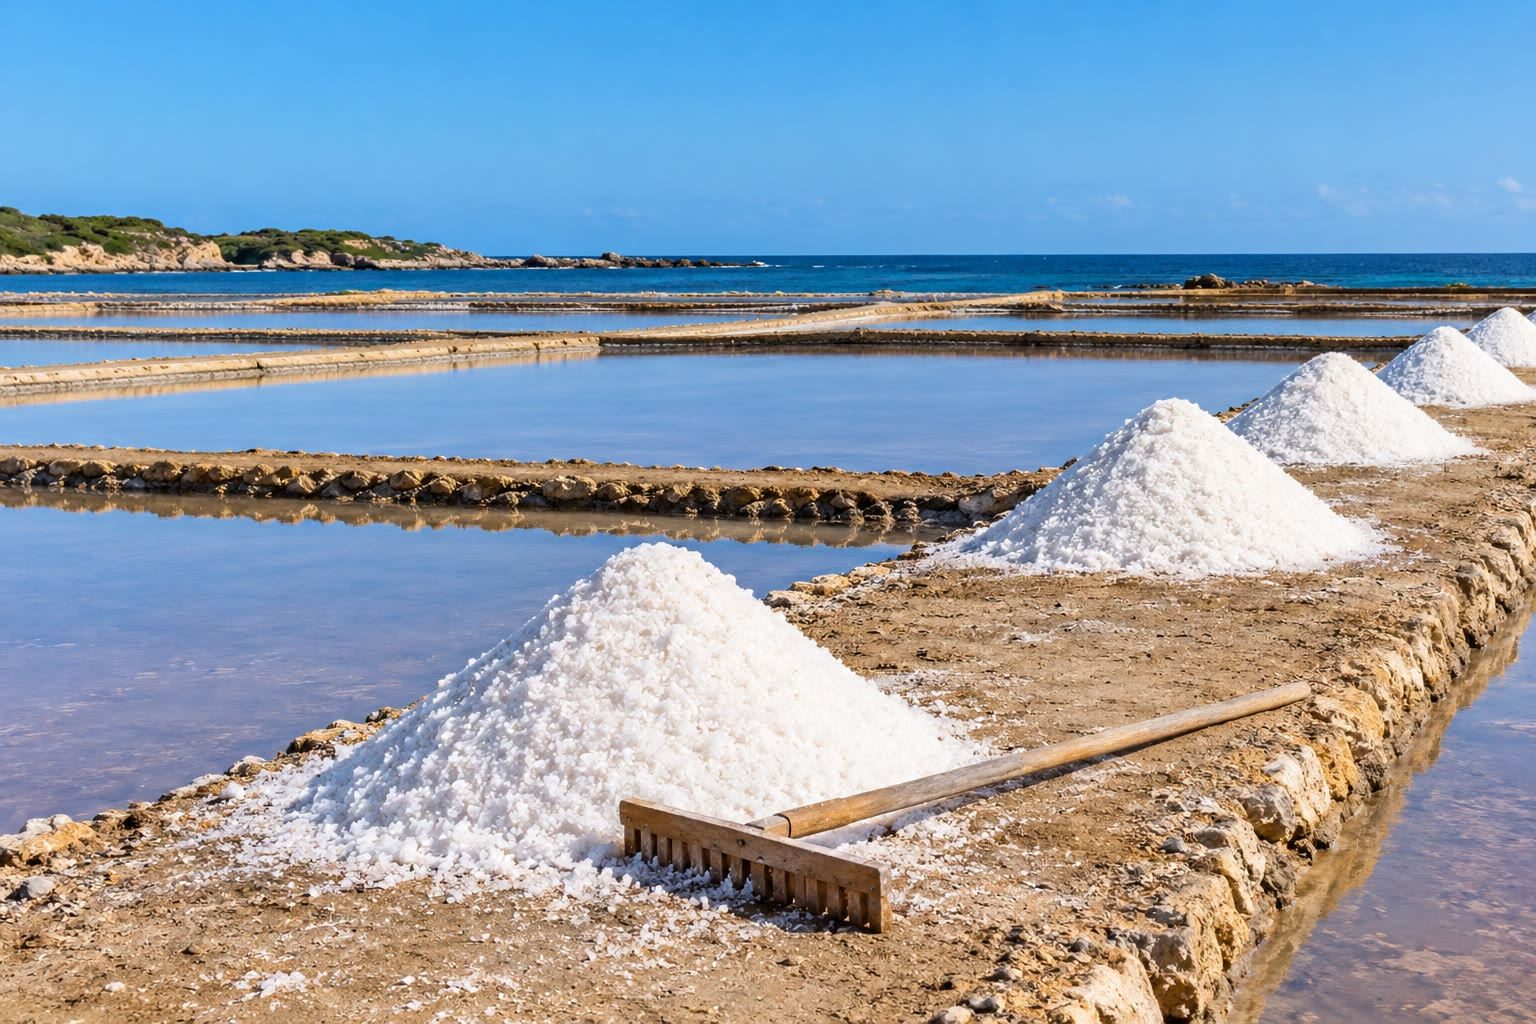
\includegraphics[width=0.62\linewidth]{images/book1/ai/g2-salt-pans.jpg}

{\small समुद्र किनारे नमक के तालाब: धूप पानी को सुखाती है, नमक सफ़ेद
ढेरों में बचा रहता है।}
\end{omfigure}

\begin{remark}[घुलना पिघलना नहीं है]\label{rem:g2:mixing-and-dissolving:not-melting}
लोग अक्सर कहते हैं कि चीनी चाय में ``पिघल'' गई। ऐसा नहीं है: पिघलना
वह है जो धूप में बर्फ़ का टुकड़ा करता है --- बिना किसी पानी के, अपने आप
द्रव बन जाना। चाय में चीनी को पानी चाहिए, और चीनी फैलकर अब भी उसमें
मौजूद है। सही शब्द है \emph{\omterm{def:g2:mixing-and-dissolving:dissolve}{घुलना}}।
\end{remark}

\section{अभ्यास}

\begin{exercise}[$\star$]\label{exo:g2:mixing-and-dissolving:1}
इनमें से कौन-से ठोस पानी में \omterm{def:g2:mixing-and-dissolving:dissolve}{घुलते} हैं और कौन-से नहीं? चीनी,
रेत, नमक, खड़िया, कंकड़।
\end{exercise}

\begin{exercise}[$\star$]\label{exo:g2:mixing-and-dissolving:2}
\omterm{def:g2:mixing-and-dissolving:dissolve}{विलयन} क्या है? इस अध्याय से दो उदाहरण दो।
\end{exercise}

\begin{exercise}[$\star$]\label{exo:g2:mixing-and-dissolving:3}
क्या मूसली की कटोरी एक मिश्रण है? क्या तुम अब भी उसका हर हिस्सा देख सकते हो?
\end{exercise}

\begin{exercise}[$\star$]\label{exo:g2:mixing-and-dissolving:4}
पानी के एक गिलास में कोई सफ़ेद चूर्ण मिलाकर चलाया जाता है। कुछ मिनट बाद
पानी धुँधला है और तली में एक सफ़ेद परत बन गई है। क्या चूर्ण घुल गया
है? \cref{met:g2:mixing-and-dissolving:test} की मदद से
समझाओ।
\end{exercise}

\begin{exercise}[$\star$]\label{exo:g2:mixing-and-dissolving:5}
शरबत वाले पानी का एक गिलास गुलाबी है। क्या वह स्वच्छ है? क्या वह रंगहीन है? क्या वह
\omterm{def:g2:mixing-and-dissolving:dissolve}{विलयन} है?
\end{exercise}

\begin{exercise}[$\star$]\label{exo:g2:mixing-and-dissolving:6}
चलाने के बाद चाय के प्याले में चीनी नहीं दिखती। वह सुराग़ बताओ जिससे
पता चलता है कि चीनी अब भी वहीं है।
\end{exercise}

\begin{exercise}[$\star$]\label{exo:g2:mixing-and-dissolving:7}
नमक के तालाबों में धूप क्या ले जाती है, और पीछे क्या
रह जाता है?
\end{exercise}

\begin{exercise}[$\star$]\label{exo:g2:mixing-and-dissolving:8}
टॉम कहता है: ``मेरी चाय में चीनी पिघल गई।'' उसे इसकी जगह कौन-सा शब्द
बोलना चाहिए, और क्यों?
\end{exercise}

\begin{exercise}[$\star\star$]\label{exo:g2:mixing-and-dissolving:9}
दो बीकरों वाला चित्र देखो। नीचे लिखे शब्द पढ़े बिना तुम कैसे बताओगे
कि किस बीकर में रेत है?
\end{exercise}

\begin{exercise}[$\star\star$]\label{exo:g2:mixing-and-dissolving:10}
नल के पानी की एक बूँद काली प्लेट पर सूखती है और एक छोटा सफ़ेद छल्ला
छोड़ जाती है। इससे नल के पानी के बारे में क्या पता चलता है?
\end{exercise}

\begin{exercise}[$\star\star$]\label{exo:g2:mixing-and-dissolving:11}
प्रयोगशाला में एक शिक्षिका के पास स्वच्छ, रंगहीन द्रव से भरे दो गिलास हैं:
एक में शुद्ध पानी है, दूसरे में नमकीन पानी। उन्हें कोई चख नहीं सकता।
वह कैसे पता करेगी कि कौन-सा कौन-सा है?
\end{exercise}
